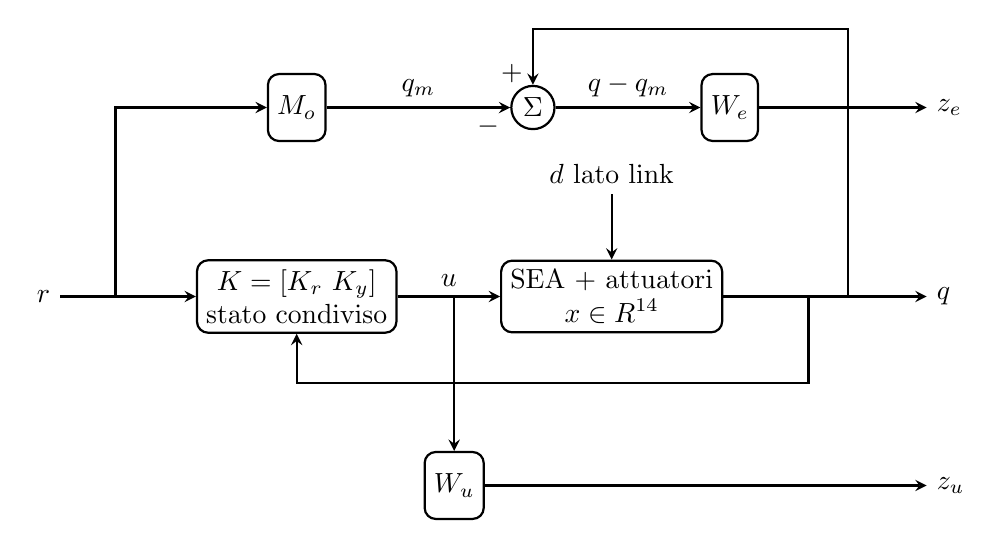
\begin{tikzpicture}[>=stealth,thick,b/.style={draw,rounded corners,align=center,minimum height=.85cm}]
\node[b] (k) at (0,0) {$K=[K_r\ K_y]$\\stato condiviso};
\node[b] (g) at (4,0) {SEA + attuatori\\$x\in\mathbb R^{14}$};
\draw[->] (-3,0)node[left]{$r$}--(k);
\draw[->] (k)--node[above]{$u$}(g);
\draw[->] (g)--(8,0)node[right]{$q$};
\draw[->] (6.5,0)--(6.5,-1.1)--(0,-1.1)--(k);
\draw[->] (4,1.3)node[above]{$d$ lato link}--(g);
\node[b] (mo) at (0,2.4) {$M_o$};
\node[draw,circle,inner sep=2pt] (sum) at (3,2.4) {$\Sigma$};
\node[b] (we) at (5.5,2.4) {$W_e$};
\draw[->] (-2.3,0)--(-2.3,2.4)--(mo);
\draw[->] (mo)--node[above]{$q_m$}node[below,pos=.88]{$-$}(sum);
\draw[->] (7,0)--(7,3.4)--(3,3.4)--node[left,pos=.8]{$+$}(sum);
\draw[->] (sum)--node[above]{$q-q_m$}(we);
\draw[->] (we)--(8,2.4)node[right]{$z_e$};
\node[b] (wu) at (2,-2.4) {$W_u$};
\draw[->] (2,0)--(wu);
\draw[->] (wu)--(8,-2.4)node[right]{$z_u$};
\end{tikzpicture}
